\chapter{Aspekte eines Anmeldesystemes und Biometrie}
\strahlhofer

\section{Prozesse eines Anmeldevorgangs}
\begin{center}
\begin{figure}[h]
    \centering
    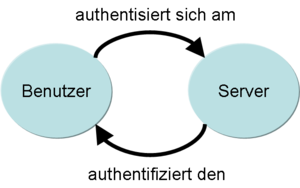
\includegraphics[width=9cm]{authentisieren-authentifizieren.png}
    \caption{Ablauf eines Anmeldevorgangs}
\end{figure}
\end{center}

%https://www.dr-datenschutz.de/authentisierung-authentifizierung-und-autorisierung/
\subsection{Authentisierung}
Bei der Authentisierung muss von einer Person ein Nachweis gegeben werden, dass sie die Person ist die sie behauptet zu sein. Dieser Nachweis kann durch drei verschiedene Methoden nachgewiesen werden, diese sind:
\begin{itemize}
	\item Die Person besitzt Wissen über eine Information, die nur der Kontoinhaber wissen kann, z.B. das Passwort oder Sicherheitsfragen sein.
	\item Das Individuum das sich versucht anzumelden und sendet beispielsweise einen Reisepass oder Führerschein als Konformation.
	\item Es wird vom Nutzer eine Information mitgesendet die er oder sie nur von sich selbst senden kann. Ein Beispiel wäre die Sendung von einem biometrischen Nachweis, dass kann entweder ein Fingerabdruck oder ein Gesichtsscan sein.
\end{itemize}

%https://www.dr-datenschutz.de/authentisierung-authentifizierung-und-autorisierung/
\subsection{Authentifizierung}
Bei diesem Schritt des Anmeldeablaufs, wird eine Überprüfung durchgeführt. Diese Prüfung soll analysiert die Informationen, die bei der Authentisierung erfasst worden sind. Können diese dem Zielkonto zugewiesen werden, dann ist der Nutzer die Person die er angibt zu sein.

%https://www.dr-datenschutz.de/authentisierung-authentifizierung-und-autorisierung/
\subsection{Autorisierung}
Die Autorisierung hat als Funktionalität die Bestätigung von bestimmten Rechten und Rollen zu bestimmten Ressourcen. Dieses Thema gehört der Informationssicherheit an und befasst sich mit der Zugriffskontrolle. Bei der Autorisierung wird für das Unternehmen ein Zugriffsmechanismus implementiert. Wenn z.B. ein Promoter sich in einem von der Firma erstellten System anmeldet, werden bestimmte Rollen und Rechte zugewiesen. Dies bedeutet das der Mitarbeiter nur einen bestimmten Zugriff auf gewisse Funktionalität besitzt.

\subsubsection{Rollen}
Bei der Anmeldung in die EMS-Software soll zwischen den Rollen Promoter und Administrator unterschieden werden. 
\begin{itemize}
	\item \textbf{Administratoren:} Die Rolle ist eine der wichtigsten in der Software. Dieser kann Benutzer und Events in einem System erstellen, verändern und löschen. Benutzer können zusätzlich deaktiviert werden, da diese entweder zu häufig falsche Anmeldeinformationen eingegeben haben oder weil die Person eine Anfrage darauf gestellt hat.
	\item \textbf{Promoter:} Diese Rolle sind Benutzer der Software, die Karten anfordern und verkaufen können. Sie können, beispielsweise die Funktionalitäten wie die Benutzer- und Eventverwaltung nicht bedienen.
\end{itemize}

%https://www.kaspersky.de/resource-center/definitions/biometrics
%Biometrie
\section{Biometrie}
%https://en.wikipedia.org/wiki/Biometrics
\subsection{Definition}
\begin{center}
	\textit{Biometrics are body measurements and calculations related to human characteristics}
\end{center}

Bei dieser Wissenschaft, schließt eine biometrische Identifikation nur auf eine bestimmte Person.
Durch diesen Aspekt ist die Biometrie eine sehr angesehne Technik in der Identifikation von Menschen.

\subsection{Methoden in der Biometrie}
Eine biometrische Information kann durch viele unterschiedliche Methoden erhoben werden.
\begin{itemize}
	%https://www.livescience.com/62690-how-dna-ancestry-23andme-tests-work.html
	%https://www.ibia.org/biometrics-and-identity/biometric-technologies/dna#:~:text=DNA%20Biometrics,often%20in%20forensics%20and%20healthcare.&text=A%20feature%20of%20DNA%20identification,familial%20relationships%20via%20DNA%20testing.
	\item \textbf{DNA-Tests:} Ein DNA-Test wird in den unterschiedlichsten Arbeitsbereichen verwendet, z.B. in der Fornesik oder von der Polizei.
	Vorteile die DNA als biometrisches Mittel zu erwägen:
	\begin{itemize}
		\item Mit der DNA kann von einer unbekannten Person auf dessen Verwandten schließen. Dies ist die einzige biometrische Methode die diese Möglichkeit bietet.
		\item DNA Spuren und Fingerabdrücke können bei Tatorten gefunden werden. Diese Methode hilft Ermittlern schneller die Identität einer Person herauszufinden.
	\end{itemize}
	%https://de.wikipedia.org/wiki/Fingerabdruck
	\item \textbf{Fingerabdruck:} Die Fingerabdrücke sind bei jedem Menschen unterschiedlich. 
	Es gibt bis zum heutigen Tag keine bewissenen Fingerabdruckstest der auf zwei verschiedene Menschen schließen konnte. 
	Nicht einmal eineiige Zwillinge besitzen den gleichen Abdruck.
	Dieser Aspekt macht diese Methode so genau, es wird hier von einer Einzigartigkeit gesprochen.
	\paragraph{Vorteile}
	\begin{itemize}
		\item Wie schon beschrieben werden Fingerabdrücke von Ermittlern verwendet, um die Identität von Opfern oder verdächtigen Personen aufzudecken.
		\item Der Fingerabdruck wird bei den meisten Smartphones in der heutigen Zeit per eingebauten Scanner ermittelt. Diese biometrischen Informationen werden erhoben um das Gerät einer bestimmten Person oder auch Personen zuzuordnen.
	\end{itemize}
	\paragraph{Nachteile}
	\begin{itemize}
		\item In dem Fall das einer Person sich auf dem Finger verletzt, kann es dazu führen das der Fingerabdruck sich verändert. Aus diesem Grund kann sich die Person möglicherweise nicht mehr identifizieren.
	\end{itemize}
	%https://en.wikipedia.org/wiki/Facial_recognition_system
	%https://www.pcs.com/wissens-werte/biometrie/gesichtserkennung-von-angesicht-zu-angesicht#:~:text=Hohe%20Sicherheit%20ist%20mit%20Gesichtserkennung,in%20der%20Regel%20nicht%20erkannt.
	\item \textbf{Gesichtserkennung:} Hier wird ein Foto oder Video analysiert und überprüft ob diese Person mit den schon aufgenommenen Bildern in der Dantebank übereinstimmen. Hier werden Aspekte wir Abstand von Augen-Nase-Mund festgestellt.
	\paragraph{Vorteile}
	\begin{itemize}
		\item Eine Person hat keinen oder kaum einen Aufwand um sich bei dieser Methode zu identifizieren. Bei Smartphones muss man lediglich in die Frontal Kamera schauen.
		\item Gesichtserkennungssysteme besitzen den Vorteil mehrere Personen aufeinmal zu erkennen. Beispielsweise in einem Labor dürfen nur bestimmte Personen zutreten. Wenn zwei Personen nun gleichzeitig eintreten wollen und einer die Berechtigung dazu nicht besitzt, wird ein Alarm ausgelöst.
	\end{itemize}
	\paragraph{Nachteile}
	\begin{itemize}
		\item Eineiige Zwillinge können bei dieser Methode schwer unterschieden werden, da diese über ein fast identisches Gesicht besitzen.
	\end{itemize}
\end{itemize}

%https://en.wikipedia.org/wiki/Touch_ID
\subsection{Fingerabdruckscans bei Smartphones}


\subsection{Gesichtserkennung bei Smartphones}

%iOS - Touchid
%Android - Fingerprint
%iOS - Face id
%Anroid - Facial Regcognition

%Sicherheit
%Genauigkeit
%Kosten
%Akzeptanz